\section{Use Case: Videoaufzeichnung}
\label{sec:Videoaufzeichnung}

Zunächst sollen im Folgenden die Grundlagen der digitalen Videoaufzeichnung und die dabei wichtigen Parameter erläutert werden.
Eine digitale Videoaufzeichnung besteht im Wesentlichen aus einer Folge von Bildern und eventuell einer Tonspur.
In dieser Arbeit liegt der Fokus auf der visuellen Komponente der Videoaufzeichnung.
Digitalkameras, wie sie auch in Smartphones zu finden sind, verwenden zur Aufnahme der einzelnen Bilder einen oder mehrere \ac{CCD} oder \ac{CMOS} Sensoren.
Diese Sensoren verwenden den Photoeffekt, um einfallende Lichtintensität in elektronische Signale umzuwandeln.
Jeder Sensor besteht aus einem Raster kleiner, als Pixel bezeichnete, Sensorelemente.
Die Lichtintensität an jedem einzelnen Pixel wird zu einem Digitalbild kombiniert \cite[S. 63ff.]{Szeliski_ComputerVision}.
Um Farbbilder zu gewinnen wird heute meist ein Sensor mit einer Bayer-Matrix, einem Muster aus Farbfiltern, verwendet.
So ist jeder Pixel nur für jeweils eine der Grundfarben Rot, Grün oder Blau zuständig \cite[S. 420ff.]{Schmidt_Videotechnik}.
Um ein nutzbares Bild zu erhalten, ist nach der Gewinnung der Signalpegel der einzelnen Pixel ein mehrstufiger Prozess notwendig.
Zum Beispiel muss zunächst Analog-Digital-Umwandlung durchgeführt werden, um die Signale in binäre Zahlen umzuwandeln, die dann weiterverarbeitet werden können.
Bei Verwendung eines Sensors mit einer Bayer-Matrix müssen die Farbwerte für jeden einzelnen Pixel beim Demosaicing aus angrenzenden Pixeln berechnet werden.
Außerdem werden oft verschiedene Prozesse verwendet, um die Qualität der resultierenden Bilder zu verbessern \cite[S. 63ff.]{Szeliski_ComputerVision}.
In \autoref{fig:ImagePipeline} ist der übliche Weg vom einfallenden Licht bis zu einem nutzbaren Digitalbild dargestellt. 
Der Prozess für die Videoaufzeichnung läuft allgemein sehr ähnlich ab.
\begin{figure}
    \centering
    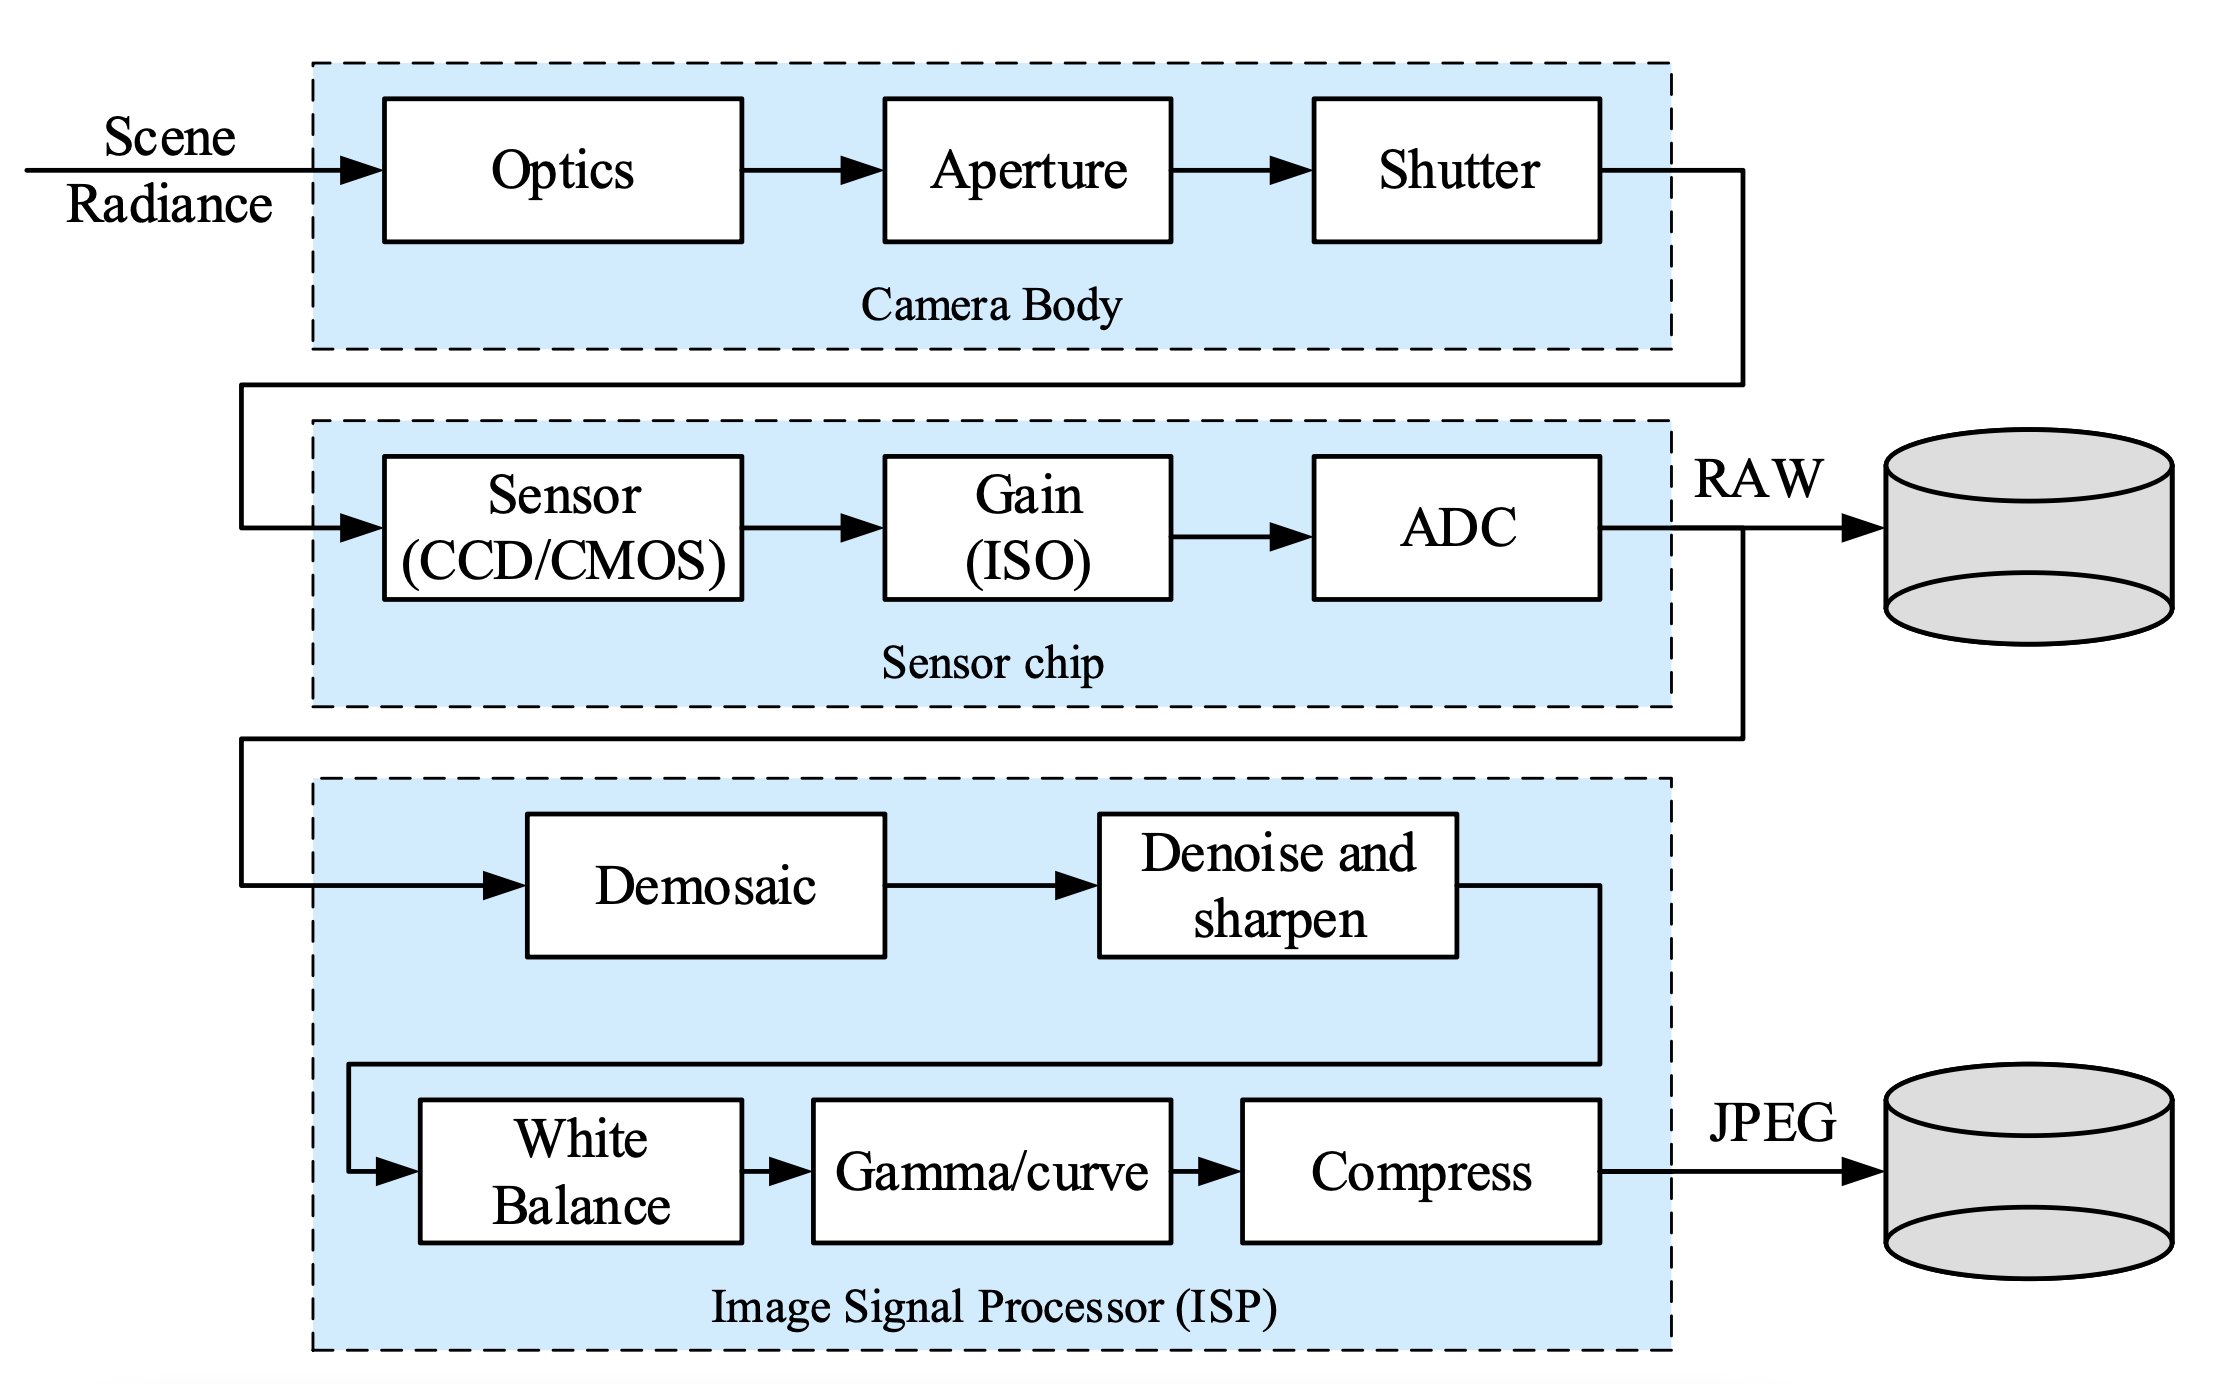
\includegraphics[width=0.9\textwidth]{ImagePipeline}
    \caption{Überblick über den Prozess der Entstehung eines Digitalbildes \cite[S. 64ff.]{Szeliski_ComputerVision}.}
    \label{fig:ImagePipeline}
\end{figure}


Das von einer digitalen Kamera aufgenommene Bild ist insbesondere von der Lichtintensität abhängig.
Diese wird vor allem durch die Belichtungszeit und die Größe der Blendenöffnung bestimmt.
Außerdem kann das Bild durch Variation der Sensorempfindlichkeit beeinflusst werden.
Die Belichtungszeit ist die Zeit, die der Sensor dem einfallenden Licht ausgesetzt ist \cite[S. 390ff.]{Schmidt_Videotechnik}.
Sensorempfindlichkeit bestimmt insbesondere die Verstärkung der elektronischen Signale und wird heute meist als \acs{ISO}-Wert, angelehnt an den zugrundeliegenden Standard der \acf{ISO}, angegeben \cite[S. 412ff.]{Schmidt_Videotechnik}.
Die Blendenöffnung ist der Durchmesser der variablen Blende, welche die Öffnung bestimmt, durch die das Licht auf den Sensor fällt \cite[S. 444ff.]{Schmidt_Videotechnik}.
Die Parameter Blendenöffnung, Belichtungszeit und Sensorempfindlichkeit werden auch als Belichtungsparameter bezeichnet.

Neben den Parametern für die Belichtung wird das Bild auch durch das verwendete Objektiv, vor allem durch Brennweite und den Fokus bestimmt.
Durch Veränderung der Brennweite lässt sich der Bildausschnitt verändern und eine Vergrößerung beziehungsweise Verkleinerung von Objekten erreichen.
Der Fokus bestimmt, welche Entfernung des Bildes scharf dargestellt wird und wird in Amateurkameras häufig automatisch eingestellt.
Die Kameras in heutigen Smartphones sind üblicherweise mit mehreren Sensoren ausgestattet, die jeweils über ein eigenes Objektiv mit unterschiedlichen Brennweiten verfügen \cite[S. 499ff.]{Schmidt_Videotechnik}.

Auch der Weißabgleich beeinflusst das Aussehen des resultierenden Bildes.
Der Weißabgleich bestimmt die Farbtemperatur des Bildes und hat insbesondere die Aufgabe unabhängig von der Lichtquelle einen gleichmäßigen Farbeindruck zu erreichen.
In Smartphone-Kameras wird er zusammen mit den meisten anderen Parametern automatisch gesetzt.
Im professionellen Bereich ist es aber oft wünschenswert einen bestimmten Wert einzustellen \cite[S. 434ff.]{Schmidt_Videotechnik}.


Bei Videoaufzeichnungen kommen weitere Parameter hinzu, welche eingestellt werden können, um das finale Video beeinflussen.
Die wichtigsten dieser Parameter sind die Bildrate, das Kompressionsverfahren und das Bildformat.
Unabhängig vom Format und der Auflösung des Sensors bieten Kameras meist die Möglichkeit das Bildformat und damit die genutzte Fläche des Sensors und die Auflösung des resultierenden Videos zu beeinflussen \cite[S. 422]{Schmidt_Videotechnik}.
Zum Beispiel werden verschiedene Formate für verschiedene Auswertungsmedien wie Kino oder TV bevorzugt.
Die Bildrate gibt an, wie viele Bilder pro Sekunde aufgezeichnet werden und beeinflusst so vor allem die Bewegungsunschärfe.
Bei schnellen Bewegungen wirken bewegte Objekte in Aufnahmen mit niedriger Bildrate unscharf.
Die Bildrate wird allerdings häufig auch als kreatives Gestaltungsmittel eingesetzt, weshalb viele Filme trotz höherer Bewegungsunschärfe mit 24 Bildern pro Sekunde produziert werden \cite[S. 174f.]{Schmidt_Videotechnik}.

Bei der Wahl von Kompressionsverfahren und Bitrate spielt sowohl der verfügbare Speicherplatz als auch die gewünschte Qualität eine Rolle.
Allgemein geht bei niedrigerer Bitrate durch stärkere Kompression mehr Qualität auf Kosten des Speicherplatzes verloren.
Allerdings sind Qualität und Speicherplatzverbrauch stark vom eingesetzten Kompressionsverfahren abhängig.
Modernere Verfahren, wie H.265 oder AV1 erreichen bei gleicher Bitrate und gleichem Speicherbedarf eine höhere Qualität als ältere Verfahren wie H.264.
Umgekehrt kann der für die gleiche Qualität benötigte Speicherplatz reduziert werden \cite[S. 253ff.]{Schmidt_Videotechnik}. 

\subsection{Für Videoaufzeichnungsapp relevante Parameter}
\label{sec:relevante_parameter}

Auf Basis der zuvor beschriebenen Parameter werden hier diejenigen Parameter identifiziert, welche im Rahmen einer Videoaufzeichnungsapp relevant sind.
Außerdem wird geklärt, welche der Parameter über die \acp{API} von iOS und Android einstellbar sind und damit prinzipiell gesteuert werden können.
Inwiefern diese Parameter auch durch die jeweiligen Cross-Plattform Frameworks eingestellt werden können, wird im Laufe dieser Arbeit geklärt.

% Welche Parameter sind prinzipiell bei Smartphones anpassbar, welche nicht